\documentclass[a4paper,twoside]{article}

\usepackage{epsfig}
\usepackage{subfigure}
\usepackage{calc}
\usepackage{amssymb}
\usepackage{amstext}
\usepackage{amsmath}
\usepackage{amsthm}
\usepackage{multicol}
\usepackage{pslatex}
\usepackage{apalike}
\usepackage{SCITEPRESS}     % Please add other packages that you may need BEFORE the SCITEPRESS.sty package.

\subfigtopskip=0pt
\subfigcapskip=0pt
\subfigbottomskip=0pt

\usepackage{graphicx,grffile}

\graphicspath{{img/}}

% *** CITATION PACKAGES ***
%
\usepackage{cite}

\usepackage{stfloats}
% *** PDF, URL AND HYPERLINK PACKAGES ***
%
\usepackage{url}

% correct bad hyphenation here
\hyphenation{op-tical net-works semi-conduc-tor}


\begin{document}

% paper title

\title{Mining of Keystroke and Mouse Dynamics to Increase the Engagement of Students with Programming Assignments}

\author{\authorname{Mario Garcia Valdez\sup{1}, Juan-J. Merelo\sup{2}, Amaury Hernandez Aguila\sup{1} and Alejandra Mancilla Soto\sup{1}}
\affiliation{Dept. of Graduate Studies, Instituto Tecnologico de Tijuana (Mexico),  \email{\tt \(mario,amherag,alejandra.mancilla\)@tectijuana.edu.mx}}
\affiliation{Geneura Team and CITIC, University of Granada (Spain),
    \email{\tt jmerelo@ugr.es}}
}

\keywords{Affective computing, neural networks, machine learning, learning analytics}

\abstract{The aim of the experiments described in this paper is to
evaluate the use of keyboard and mouse dynamics as an appropriate
non-obtrusive sensory input for an system that is sensitive to the
affective state of its user. Our motivation for starting this research
line has been the lack of tools and methodologies for taking into
account this affective state in learning
environments. In an ideal situation, when instructors have to choose
from  a collection of programming assignments, they should consider the
  student\'s affective state and skills in order to select a learning resource
  with the appropriate level of difficulty. However, neither the data
  or the ability to process it are present in current learning
  management systems. This work tries to address this problem, by
  focused on the capture and pre-processing of data that is going to
  be fed to several machine learning techniques with the objective of classifying the affective
states of users with different levels of expertise
when learning a new programming language. We capture student data from
a web-based platform, a learning management system where students
interact whith programming excersises. We introduce in this paper a
series of pre-processing techniques that are able to convert data from keyboard and mouse dynamics captured from students as
they were coding basic Python programming assignments  into feature
vector, that have been later used for the classification into five affective states:
boredom, frustration, distraction, relaxation and engagement.
The following classification algorithms have been evaluated: k-nearest
neighbors,feed forward neural networks, na\"ive Bayes classifier, J-48
tree induction algorithm, deep learning, random forest, gradient boosted trees and na\"ive Bayes Kernel). The best accuracy was around 78\% and was achieved
by the tree induction algorithms. Results show that data gathered from ready-available,
non-obtrusive sensors can be used successfully
as another input to hyebrid classification models in order to predict an
individual\'s affective states, and these in turn can be used to make
students more engaged and thus learn more efficiently.}

\onecolumn \maketitle \normalsize \vfill

\section{Introduction}
Programming courses are often regarded as difficult
\cite{robins2003learning, lahtinen2005study,munson2018models}
and there is a common conception, backed by data, that they often have a high
failure rate \cite{bennedsen2007failure}.
Jenkins \cite{jenkins2001motivation} argues that this high rate of failure has
multiple factors:
\begin{itemize}
\item There is a deep relation with the expectations, attitudes,
and previous experiences of the teaching staff and students.
\item The nature of the subject that involves the
learning of new abstract constructs, syntax and tools.
\item Groups are often heterogeneous and thus it is difficult to design courses
that are beneficial for everyone. Many students begin to program when they
are at their first year of university which means they are tackling a totally
new topic that does not respond to their habitual study approaches.
\end{itemize}

Dijkstra \cite{dijkstra1989cruelty} argues that the subject of programming is
very problem-solving intensive, which means that a high precision is required
since even the slightest deviation from syntax can render a program
totally worthless. These are hurdles that often frustrate novice
students. This is aggravated by the fact that the time devoted to a
particular topic is fixed, and when it is exhausted, instructors move to explain
more advanced subjects, while a group of students might still be struggling with
basic syntax.
Again Jenkins \cite{jenkins2001motivation, jenkins2002difficulty} notes that
many students expect the course to be difficult and come with the notion that
they will have to struggle; others may have a stereotyped image of a programmer,
and these beliefs can negatively affect their initial motivation and expectations.
During the duration of the course and its delivery, novice programmers
have been proved to experience  emotions such as frustration and
confusion when a bug in a program eludes them, but also joy when they
successfully run a challenging program for the first time. They can also become
bored if they found the assignments too repetitive or too easy.

Learning to program is a difficult task, and similarly to other
learning tasks, emotions play a significant
role. Research has gone far to understand the role of emotion in learning, both
in the process and the outcome; for instance, in e-learning
\cite{kort2001affective, rossin2009effects}
and in programming  \cite{rodrigo2009affective, jenkins2001motivation ,
bosch2013emotions, khan2007mood}. In these works the emotion of flow/engagement
is regarded as the ideal affective state in which
students tend to be most capable of acquiring meaningful information through the
learning process. Flow is defined by Csikszentmihalyi \cite{csikszentmihalyi1990flow}
as a mental state in which a person performing an activity is fully immersed in a feeling of energized focus, full involvement, and enjoyment. Engagement is
also a positive affect where students are thought to be more involved
behaviorally, intellectually, and emotionally in their learning tasks
\cite{bangert2002teacher}.

In order to promote engagement, sometimes instruction material is designed with the
objective of creating learning activities that are challenging to students, but
not so much as to frustrate them. Engagement is not only achieved through the
design of single learning activities but also on the appropiate selection and
sequence in which they are presented.
For this, experienced instructors gauge a student\'s affective state and then
assign an activity with the appropriate level of difficulty. However,
recognition of emotions is a difficult task, even
for humans. Instructors often use their social intelligence to recognize
students\'' affective states. During presential  classes, an instructor habitually reads the
faces of students in the classroom to see if they are confused, bored or
engaged and then decides what to do next. However, that is impossible
in asynchronous and virtual learning environments, that is why there
have been several ways of including automatic perception of emotions
in Interactive Learning Environments (ILEs) and Learning Management
Systems \cite{gottardo2017affective} and even in Integrated
Development Environments \cite{hundhausen2017ide}.

But this of course presupposes that the affective state of the student
is available to the system. This detection and recognition can be done
in real time in different ways. In the wider context of the detection
of emotions and affective 
state, many researchers have
demonstrated that affect-aware computers can provide a better performance in
assisting humans
\cite{picard2001toward,munson2018models,bosch2017affective}, and that
providing a richer experience while learning to program might improve
the outcome by making the students more engaged with it
\cite{asensio2014progamer}. However, when ILEs embrace these methodologies
and techniques a
problem arises: Sensors which are not present in the default computer
configuration must be used to gather data that will be used to perform the
recognition of users\' affective states.
Some sensors rely on physiological readings
and must be in physical contact with students \cite{atkinson2017assessing,swansianalyzing}.
These sensors can be considered
intrusive or invasive, not to mention that you have to acquire them
and convice the student to wear them while learning.  They can also disrupt the student\'s learning experience
\cite{zhai2008stress, sidney2005integrating, arroyo2009emotion}.
Other less cumbersome sensors, such as video cameras, which are in
fact default equipment in most laptops, can also be considered invasive, since
they always transmit the user's identity, appearance and behavior along with
the emotional data \cite{picard2001toward}. So what we would need in
order to embed recognition of affective states in learning systems
would be non-invasive, anonymous and also ubiquitous sensors. In this
paper we are going to test such a kind of system.

And in order to do that, we will use the dynamic of the learning
environment itself. In programming courses, students solve assignments
by implementing their solution in a particular language; in order to
do this, they must type the code, run it directly or by compiling it
to check its results. This cycle can be repeated many times, and as
they are in this cycle, studens often change their affective state
according to their performence.  Data can, then, be non-intrusively
collected while students are working on their assignments and typing
on the keyboard and interacting with the GUI via mouse or other
pointing device.  All the dynamics of actually typing the code and ILE
feedback received by students, the corrections they tried, the elapsed
time between each step, the number of attempts, compiling errors,
exceptions, among others, are collected by the ILE and can be
used. Data mining of all this data could bring us a better
understanding of the learning process, and also a better model of the
student state for both the selection of the appropriate content to be
shown next and to evaluate the learner\'s competencies. But the
problem that remains is to how to recognize the student's affective
state so that it can be used by an adaptive system.

In this work, a method for the recognition of affective states in real
time through the
mining of keystroke and mouse dynamics data is analyzed further after
its initial presentation in \cite{ijcci17}.
Since students can vary the dynamic of keystrokes according
to their affective state when programming, a correlation between the
user\'s interactions (keyboard and mouse) with an emotional state has been
established in preliminary work by Zimmermann
et al. \cite{zimmermann2003affective}, but the work experiments where
conducted by asking users to write a predefined message, not programming
exercises.
In order to test the correlation of keyboard and mouse dynamics and an
affective state when programming, an interactive web-based
programming platform was initially proposed by us in
\cite{ijcci17}. In this paper we complete the background and
motivation for this research, and update the state of the art, as well
as justify better the methdology used and the way data has been
collected, extending the results and the methods used. The platform we
presented in that paper originally was 
designed to collect keyboard and mouse data 
from the students\' interaction for data analysis. The proposed method
has three main components: a JavaScript library to capture keyboard
and mouse dynamics from a browser-based editor, a pre-processing step
whose output is a feature vector that is sent to a third component,
the classification algorithm.

An experiment was conducted where students solved a series of programming
assignments using the web based learning environment. Using only the
data from the student\'s keyboard and mouse dynamics six affective
states where recognized for each of the attempts at solving the
assignments. Results obtained from the experiment are promising. The
affective states recognized include the most common in novice
programmers according to the study of Bosch, D'Mello \& Mills
\cite{bixler2013detecting}: boredom, engagement/flow, confusion and
frustration. For the initial experiment \cite{ijcci17} 
four binary classifiers were compared: J-48 decision trees, k-nearest neighbour
classifier, feed forward neural network, and a na\"ive Bayes. The output of each
classifier determined if the student experienced the affective state during the
assignment. In this experiment we will also use 
Deep Learning \cite{candel2016deep} and  Gradient Boosted Trees 
via H2O version 3.8.2.6, and the Random Forest and Na\"ive Bayes Kernel 
implementatios from RapidMiner Studio version 8.1.

The proposed method could be used in an ensemble with other sensor
channels to improve the non-invasive recognition of the students’ affective
states when they are working on a programming task.

In order to determine what
affective states a student was experiencing, an Experience Sampling Method (ESM)
was used by Csikszentmihalyi \& Larson \cite{kubey1996experience}. After the students successfully
solve a programming assignment, they are presented with an ESM survey that asks
what they were feeling during their solving of the assignment.

If a relationship between interaction dynamics and affective state could be modeled, ILEs could adapt the instruction using the
same devices required to input the program to the computer, which
could constitute a breakthrough since writing programs in a computer
is the best way to learn programming by actually doing it. A by Lahtinen, Ala-Mutka \& Järvinen
\cite{lahtinen2005study} reports that students rated ``working alone on programming coursework'' as a more useful situation than lectures.

The rest of the paper is structured as follows: next Section presents
a series of works related to the proposed method in this paper;
Section \ref{sec:method} describes the proposed method for the
recognition of affective states in a web based learning environment
for the teaching of programming languages; next in Section
\ref{sec:exp} we explain the experimental evaluation of the proposed
method and results.  Finally, we draw some conclusions about our
methodology and experiments.


\section{Related Work}

Affect recognition is an active field of research. Many
methods have been proposed, some of them requiring the intervention of
the user to fill up questionnaires or forms; these selections remain static until the user changes
the values and are easy to implement, but cannot detect dynamic
changes.  A more dynamic approach requires the use of sensors to capture
affective states in real time, and that is what we are doing in this
paper. 

The actual sensors are determined by the context, the environment and the learning
activity determine. The most common learning
environment is the classroom, a physical space that provides a context to facilitate
learning. But learning is possible in a wide variety of settings, such as
out-of-school locations and outdoor environments which are sometimes
referred to as ubiquitous learning environments. An analysis of such
environments is done by Yang \cite{yang2006context} in a context-aware
environment, but his work misses affective information. There are also
virtual learning environments such as the one proposed by Dillenburg 
\cite{dillenbourg2002virtual}  where learners can have avatars, and virtual places
where they can play roles and socialize. In general, the importance of
affect in learning environments has been recognized at a later stage
of research. 

For instance, the work of Kapoor y Picard \cite{kapoor2005multimodal}
uses a multimodal 
approach with sensory information from facial expressions and postural shifts
of the learner combined with information about the learner\'s activity on the
computer; the learning activity was solving a puzzle on a computer. They report
using a multimodal Gaussian Process approach achieving an accuracy of over 86\%.
Sidney, et al., \cite{sidney2005integrating} enhances the intelligent tutor system AutoTutor with
affective recognition using non-intrusive sensory information from facial
expressions, gross body movements, and conversational cues from logs.  The
subject material of that system consisted in lectures of computer
literacy. In this early stage of research, the importance of privacy
and non-intrusiveness is set aside. 

Some other works try to introduce affective computing features into
interactive learning environments, without explicitly detecting of
using the student's affective state. For instance, Elliott, Rickel y Lester \cite{elliott1999lifelike,d2008autotutor}
propose the integration of an affective reasoner 
with an agent in a virtual environment. In this work an agent called Steve
responds emotionally to other agents and interactive users. The agent simulates
his emotions through different multimedia modes including facial expressions and
speech. Affective reasoning agents were used for training, by putting students
in work related situations. Agents could react to the behavior of students; for
instance if a student was being careless in a task and was in a dangerous
situation, Steve would show distress or fear. Also in a virtual environment the
work of McQuiggan, Robison \& Lester \cite{mcquiggan2010affective} extends this line of research by
investigating the affective transitions that occur throughout narrative-centered
learning experiences. The analysis of affective state transitions in this work
replicated the findings by D’Mello et al. \cite{d2008autotutor} and Baker et al.
\cite{rodrigo2009affective} where
also engagement/flow dominated self-reported affect. For outdoor environments
Shen, Wang \& Shen \cite{shen2009affective} augment a pervasive e-learning platform with affective
recognition.  The results about emotion recognition from physiological signals
achieved a best-case accuracy (86.3\%) for four types of learning emotions.

Bosch, D'Mello \& Mills \cite{bosch2013emotions} analyzed the relationship between affective states
and performance of novice programmers learning the basic Python. The results of their study
indicated that the most common emotions students experienced were engaged
(23\%), confusion (22\%), frustration (14\%), and boredom (12\%). It was useful
to consider these results, as it presented evidence of what affective states
need to be targeted in order to obtain less biased data. Similar to
the previous work, Rodrigo et al., \cite{rodrigo2009affective} observed which affective states and
behaviors relate to student\'s achievement within a basic computer science
course. The authors found that confusion, boredom and engagement in IDE-related
(on-task) conversation are associated with lower achievement. Measuring mood is important,
since it may have an impact on programmer\'s performance according
to Khan, Hierons y Brinkman \cite{khan2007mood}. It may be possible to detect moods
on the basis of information regarding the programmer\'s use of the keyboard and
mouse, and to integrate them into development environments that can improve
programmer performance.

There has been very little research reported on the effectiveness of
the use of keyboard and mouse dynamics as a sensory channel for
affective recognition, and the few have not been focused on
programming. The preliminary work by Zimmerman et
al. \cite{zimmermann2003affective} describes a method to correlate
user’s interactions (keyboard and mouse) with an emotional state,
measuring different physiological parameters. The work of Vizer, Zhou
and Sears \cite{vizer2009automated} also uses sensory data based on
the time elapsed between each key press, the task given to users was
to write a free-text and used linguistic features in order to
recognize both physical and emotional stress. The results show a
classification accuracy of 62.5\% for physical stress and 75\% from
emotional stress; authors argue that these results are comparable with
other approaches in affective computing.

They also stress that their methods must be validated further in
other contexts. Moods may have an impact on programmer\'s performance according
to Khan, Hierons and Brinkman \cite{khan2007mood}. It may be possible to detect moods
on the basis of information regarding the programmer\'s use of the keyboard and
mouse, and to integrate them into development environments that can improve
programmer performance. They briefly describe a further experiment that could
use keyboard and mouse but only as future work. There are other studies about
the behaviour of programmers, which are not directly concerned with affective
states but are nevertheless important to their performance. Eye tracking in
computing education is proposed in the work Busjahn et al., \cite{busjahn2014eye}, and it is
also used for assessing learner´s comprehension of C++ and Python programs in
Turner et al., \cite{turner2014eye}. Blikstein \cite{blikstein2011using} proposed
an automated technique to
assess, analyse and visualize students learning computer programming. Blikstein
employs different quantitative techniques to extract students’ behaviours and
categorize them in terms of programming experience.

\begin{figure*}[h!tbp]
\centering
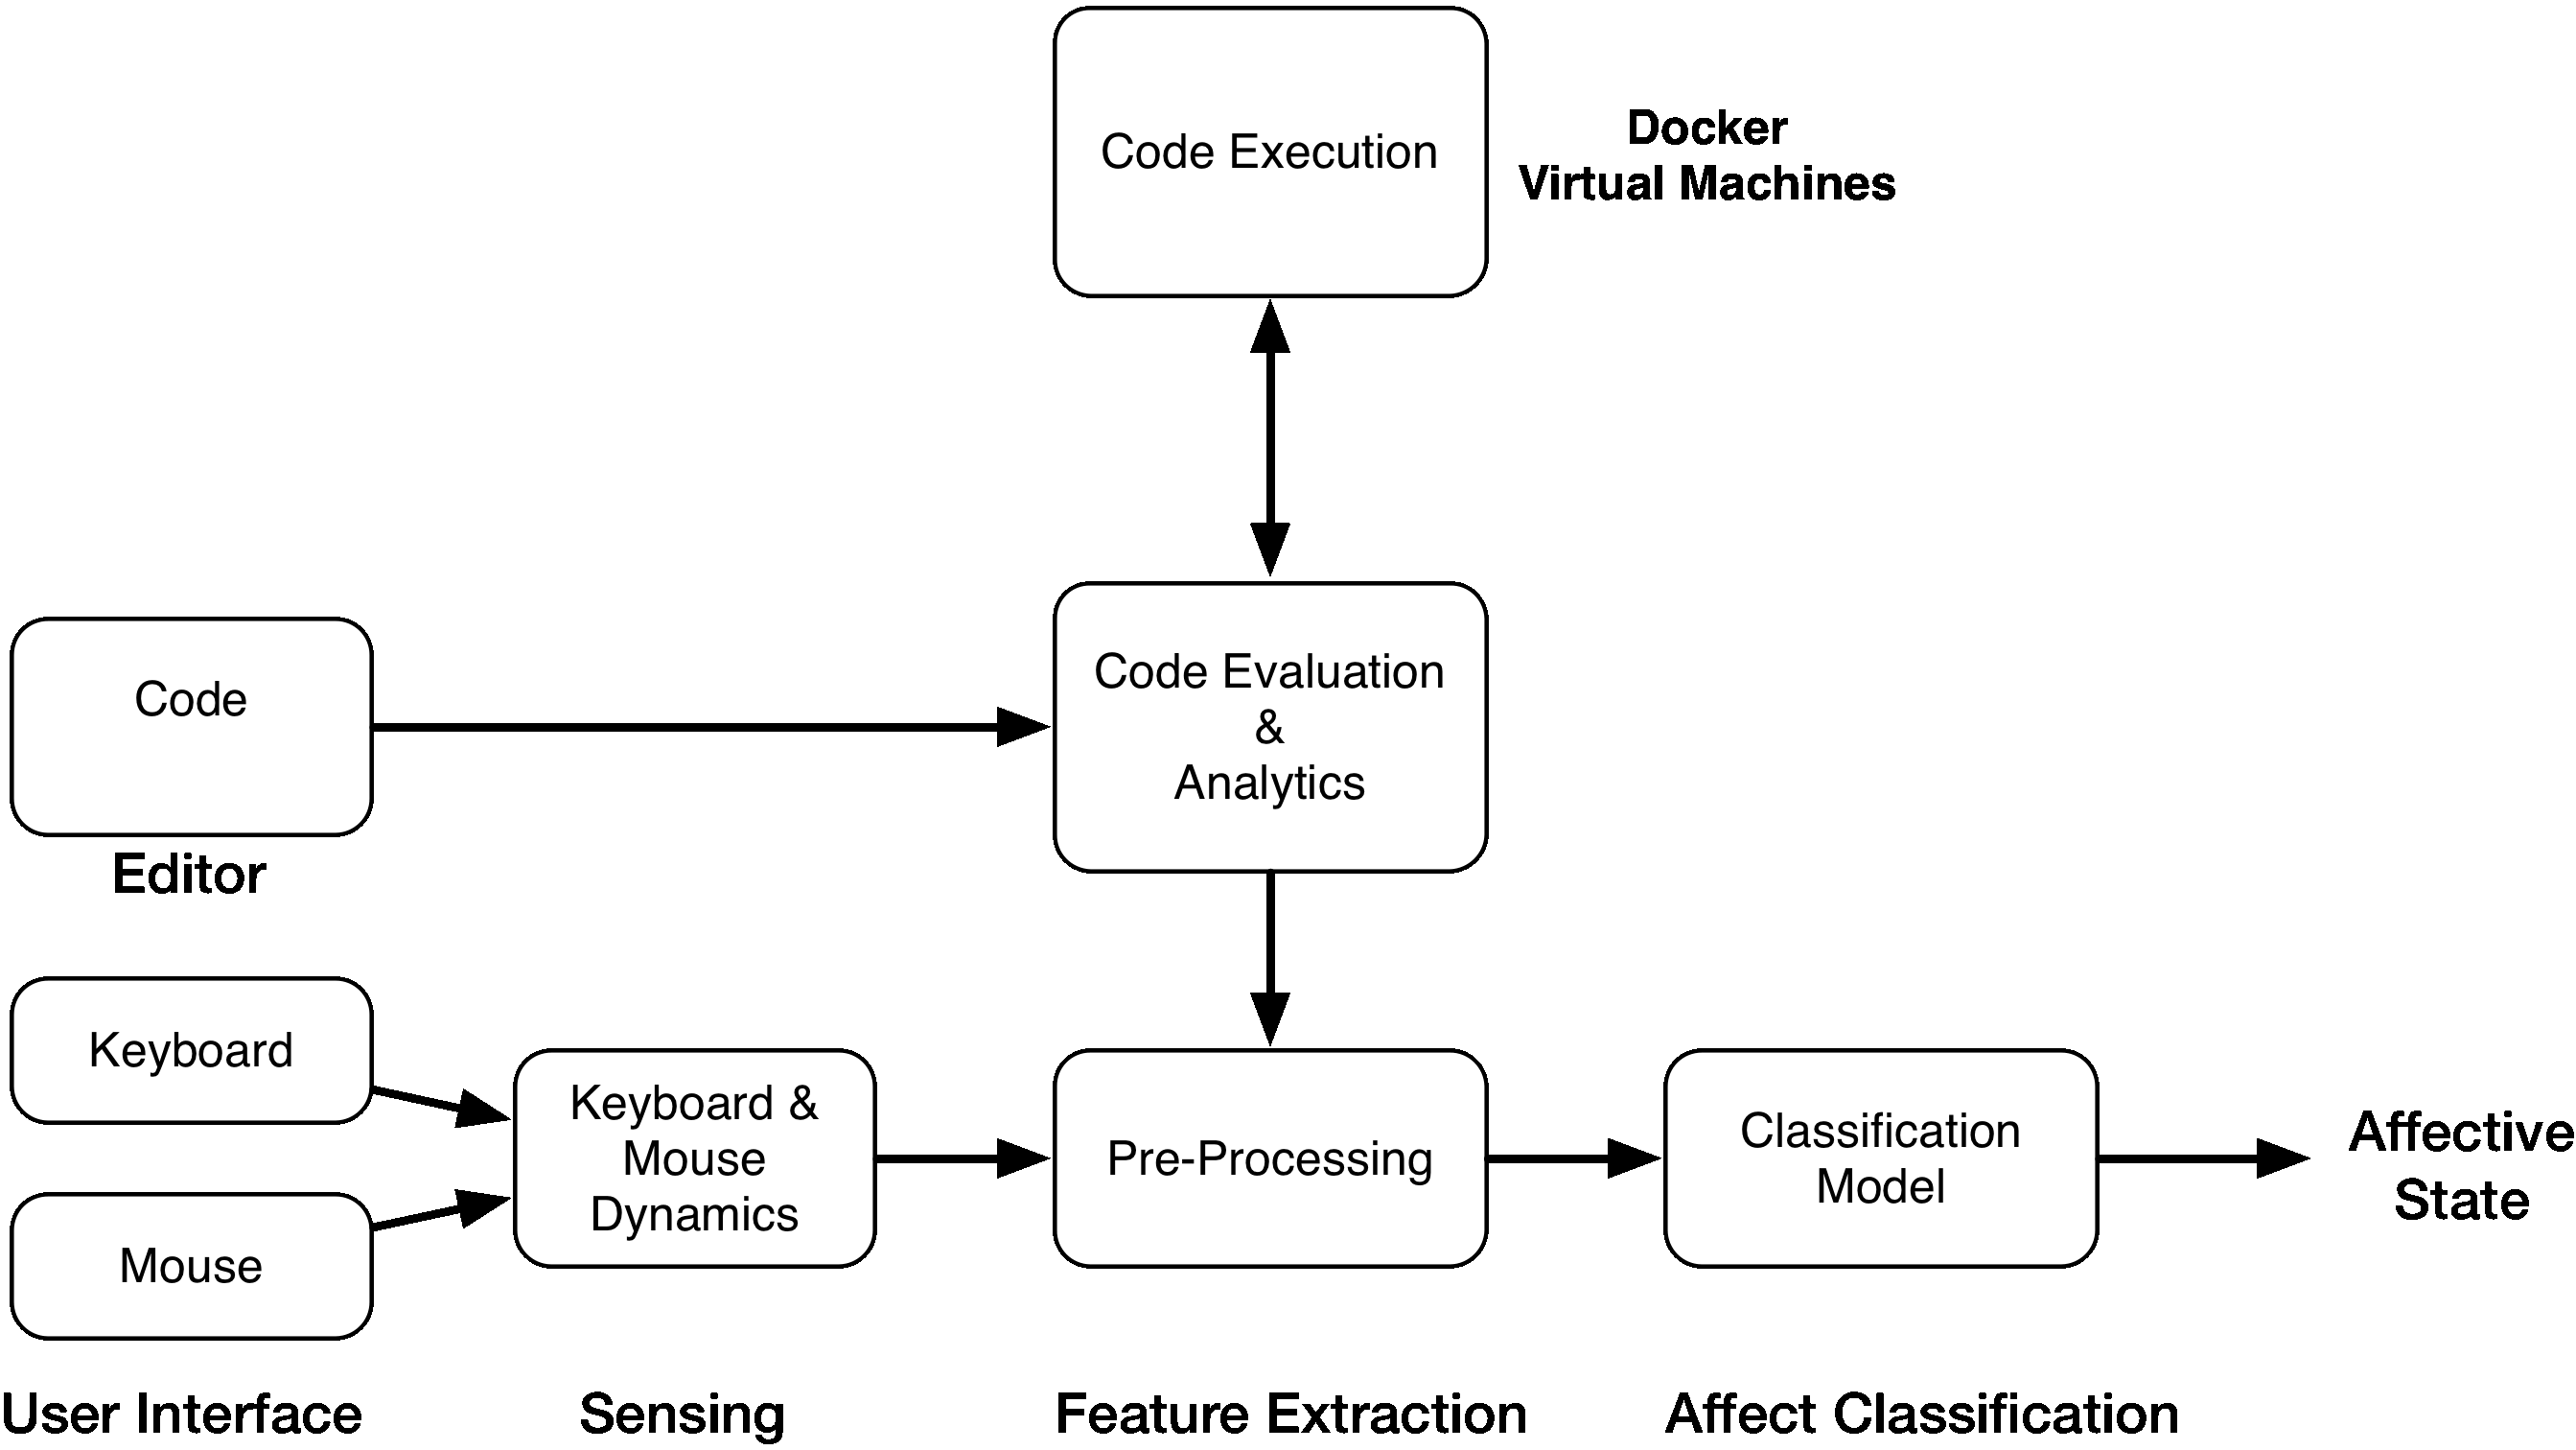
\includegraphics[width=0.80\textwidth]{KMDAffective.png}
\caption{Code Execution and Affect Recognition Architecture.}
\label{fig_process}
\end{figure*}

It is obviously necessary, in order to detect the moods, to prove that
there is an actual relationship between them and the keyboard
activity. In fact, Keystroke Dynamics (KD) has been investigated  by using either
fixed-texts or free-texts \cite{gunetti2005keystroke}.
KD performed on fixed-texts
involves the recognition of typing patterns when typing a pre-established fixed-
length text, e.g., a password. In the other case, free-text KD achieves the
recognition of typing patterns when typing a text of arbitrary-length, e.g., a
description of an item. However, as noted by Janakiraman and Sim
\cite{janakiraman2007keystroke}, most of 
the research regarding KD is done on fixed-text input, the reason being that
fixed-text KD usually yields better results than free-text KD. Yet, the authors
of this work share the opinion with Janakiraman, R., and Sim, T., that it would
 be more useful if KD can handle free text as well as fixed text, this is also a
 requirement if the text is a program. This is what we are actually
 using in this paper, since programs are created by the student and do
 not have to follow exactly the same pattern. 

Although the use of KD is found in several research works
as a biometric measure, its use for identifying affective states is rare in
comparison. Epp, Lippold \& Mandryk \cite{epp2011identifying} effectively used KD in conjunction
with decision-tree classifiers for the identification of 15 affective states.
Although their work was based on fixed text, their technique to extract a feature
vector was an inspiration for the proposed method in this work. As for free-text
KD, Bixler y D\'Mello \cite{bixler2013detecting} present a method for the identification of boredom
and engagement based on several classification models. A similar situation exists in the case of Mouse Dynamics (MD), which is used mainly for authentication; however, Salmeron-Majadas, Santos
and Boticario \cite{salmeron2014exploring} use both MD and KD to predict four affective states using
five different classification algorithms. Bakhtiyari y Husain \cite{bakhtiyari2014fuzzy} discuss a
method based on fuzzy models for the recognition of emotions through KD, MD and
touch-screen interactions. Lim \cite{lim2017detecting} use several
sensor sets and methods for detecting stress levels, including neural
networks; the detected stress level is then fed into the inference
system that decides on adaptation. However, this work focuses only on
stress level, disregarding the more general affective state. Although
it is no longer current, the state of the art was described quite
comprehensively in Kolakowska's paper \cite{kolakowska2013review}.

More recent papers, like the one by Carneiro and Novais \cite{CARNEIRO2017171} takes a
more comprehensive approach, using also a non-intrusive system based
on keystroke analysis; several affective states are measured: mental
fatigue, stress and emotional valence. However, it is not focused
particularly in programming, which has certain characteristics, but
uses music to create a certain mood on the subjects. The KD
methodology, however, is applicable to a wide range of
situations. Also Kolakowska has recently published a paper
\cite{Kolakowska2018} assessing the usefulness of KD not only in
emotion recognition, but also in user authentication. Whatever the
method, it is indeed proved that KD can be used for detecting a range
of user mood and attitudes \cite{wrobel2018applicability}. In this
paper we are more concerned with the data collection and the selection
of a particular method for detecting the mood with the limited amount
of data obtained via KD. 


\section{Proposed Method}
\label{sec:method}

The goal of this work is to propose an affective
recognition method based on the sensory data provided by the keyboard and mouse
dynamics generated by a learner as he or she types a programming assignment.
A detailed explanation of the process outlined in a previous work \cite{ijcci17} is explained next.
The process starts when the
learner begins to type a program in a browser-based editor. As she types or
moves the mouse all the data of the dynamics is recorded on the client.
When the learner submits the code to evaluation, the HTTP request includes,
in a JSON string, all the sensory data along with the code and
information about the current session.
In the web server, the code is evaluated by an
external container that provides a virtual sandbox in which to execute the
program. The sandbox is used to prevent malicious or
erroneous code to halt the server. When a container is halted, it is simply
removed and a new container is created.
When the result is ready, it is recorded
along with the sensory data and sent to the preprocessing module that it will
be explained next. The output is a feature vector, ready for classification. A
previously trained classifier is responsible for the classification, which
outputs the predicted affective state.

Currently, the method does not consider other sensory data,
but it could be integrated with other sensory inputs in a multi-modal
approach.  Each of the steps is explained in detail next.

\begin{table*}[h!tb]
\centering
\caption{The components of the feature vector; adapted from Epp, Lippold \& Mandryk \cite{epp2011identifying}.}
\label{tab_features}
    \begin{tabular}{ | l |p{0.4\textwidth} || l | p{0.4\textwidth} | }
    \hline
    ID          & Description           & ID               & Description  \\
    \hline
    1 & Mean duration between 1st and 2nd down keys of the digraphs.  & 21 & Mean duration of the 2nd key of the trigraphs.\\
    \hline
    2 & Standard deviation of the previous feature.                   & 22 & Standard deviation of the previous feature.\\
    \hline
    3 & Mean duration of the 1st key of the digraphs.                 & 23 & Mean duration between 2nd key up and next key down of trigraphs.\\
    \hline
    4 & Standard deviation of the previous feature.                   & 24 & Standard deviation of the previous feature.\\
    \hline
    5 & Mean duration between 1st key up and next key down of the digraphs. & 25 & Mean duration of the third key of the trigraphs.\\
    \hline
    6 & Standard deviation of the previous feature. & 26 & Standard deviation of the previous feature.\\
    \hline
    7 & Mean duration of the 2nd key of the digraphs. & 27 & Mean duration of the trigraphs from 1st key down to last key up.\\
    \hline
    8 & Standard deviation of the previous feature. & 28 & Standard deviation of the previous feature.\\
    \hline
    9 & Mean duration of the digraphs from 1st key down to last key up. & 29 & Mean number of key events that were part of the graph.\\
    \hline
    10 & Standard deviation of the previous feature. & 30 & Standard deviation of the previous feature.\\
    \hline
    11 & Mean number of key events that were part of the graph. & 31 & Mean duration of mouse key presses.\\
    \hline
    12 & Standard deviation of the previous feature. & 32 & Standard deviation of the previous feature.\\
    \hline
    13 & Mean duration between 1st and 2nd down keys of the trigraphs. & 33 & Mean duration of all mouse movements.\\
    \hline
    14 & Standard deviation of the previous feature. & 34 & Standard deviation of the previous feature.\\
   \hline
    15 & Mean duration of the 1st key of the trigraphs. & 35 & Mean distance in pixels in the X coordinate. \\
    \hline
    16 & Standard deviation of the previous feature. & 36 & Standard deviation of the previous feature.\\
    \hline
    17 & Mean duration between 1st key up and next key down of trigraphs. & 37 & Mean distance in pixels in the Y coordinate.\\
    \hline
    18 & Standard deviation of the previous feature. & 38 & Standard deviation of the previous feature.\\
    \hline
    19 & Mean duration between 2nd and 3rd down keys of the trigraphs. & 39 & Number of attempts\\
    \hline
    20 & Standard deviation of the previous feature. &   &  \\
    \hline
  \end{tabular}
\end{table*}

\subsection{Capturing the Keystroke and Mouse Data}
As it was explained before, as a student is trying to solve an assignment,
a script coded in JavaScript runs in the background,
capturing every keystroke, mouse movement and mouse button pressed. Each record
of these events includes a time-stamp in milliseconds (using the method
getTime() of JavaScript\'s built-in class Date) that describes when the event
occurred. If the event is a keystroke, the script captures what key was
specifically pressed, and what type of event occurred, it can be either a key-
down or a key-up event. If it is an event related to a mouse button press, the
key code of that button is recorded, as well as the type of event occurred again
key-down or key-up. Finally, if the event was a mouse movement, the mouse
coordinates inside of the web browser are recorded. The script monitors the
mouse position every 100 milliseconds, and only if the position has changed, it
records the new position. Each time a learner tries to evaluate a program, all
the data generated is sent to the server along with the code. When the result of
the execution is returned, all records are cleared and the process starts again.
There is no problem if the user leaves for a long period of time, because no
event will be triggered. If a user copies and then pastes the code from another
source, this will be recorded. There is a limitation, only the browser-editor
must be used; this could be a problem for more advanced programmers needing
specialized editors.  On the other hand a browser-based editor with the
corresponding remote execution, does not require the installation of
interpreters or compilers in learner’s computer. The code could even be written
in a mobile device or any web-enabled device. Programming assignments are
evaluated using unit tests; the results of the evaluation are shown to users.
If all tests the program is considered to be correct. The source code for the
Protoboard web based learning environment including the KD and MD functions are
open source and available as Github repositories
at\url{https://github.com/amherag/keyboard-mouse-dynamics}; the code for the
sandbox is also available in \url{https://github.com/mariosky/sandbox}.

\begin{figure*}[h!tb]
\centering
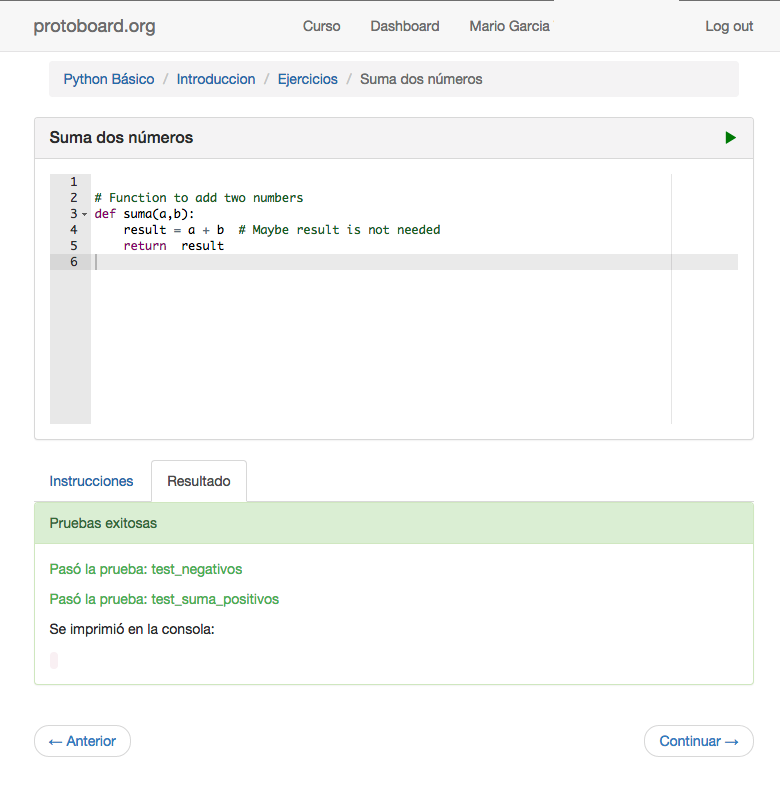
\includegraphics[width=0.60\textwidth]{editorRresult.png}
\caption{Web-based editor used for code evaluation. The lower panel
  indicates (in Spanish) the tests passed successfully and the program
  output \cite{ijcci17}.}
\label{fig_editor}
\end{figure*}

\begin{figure*}[h!tb]
\centering
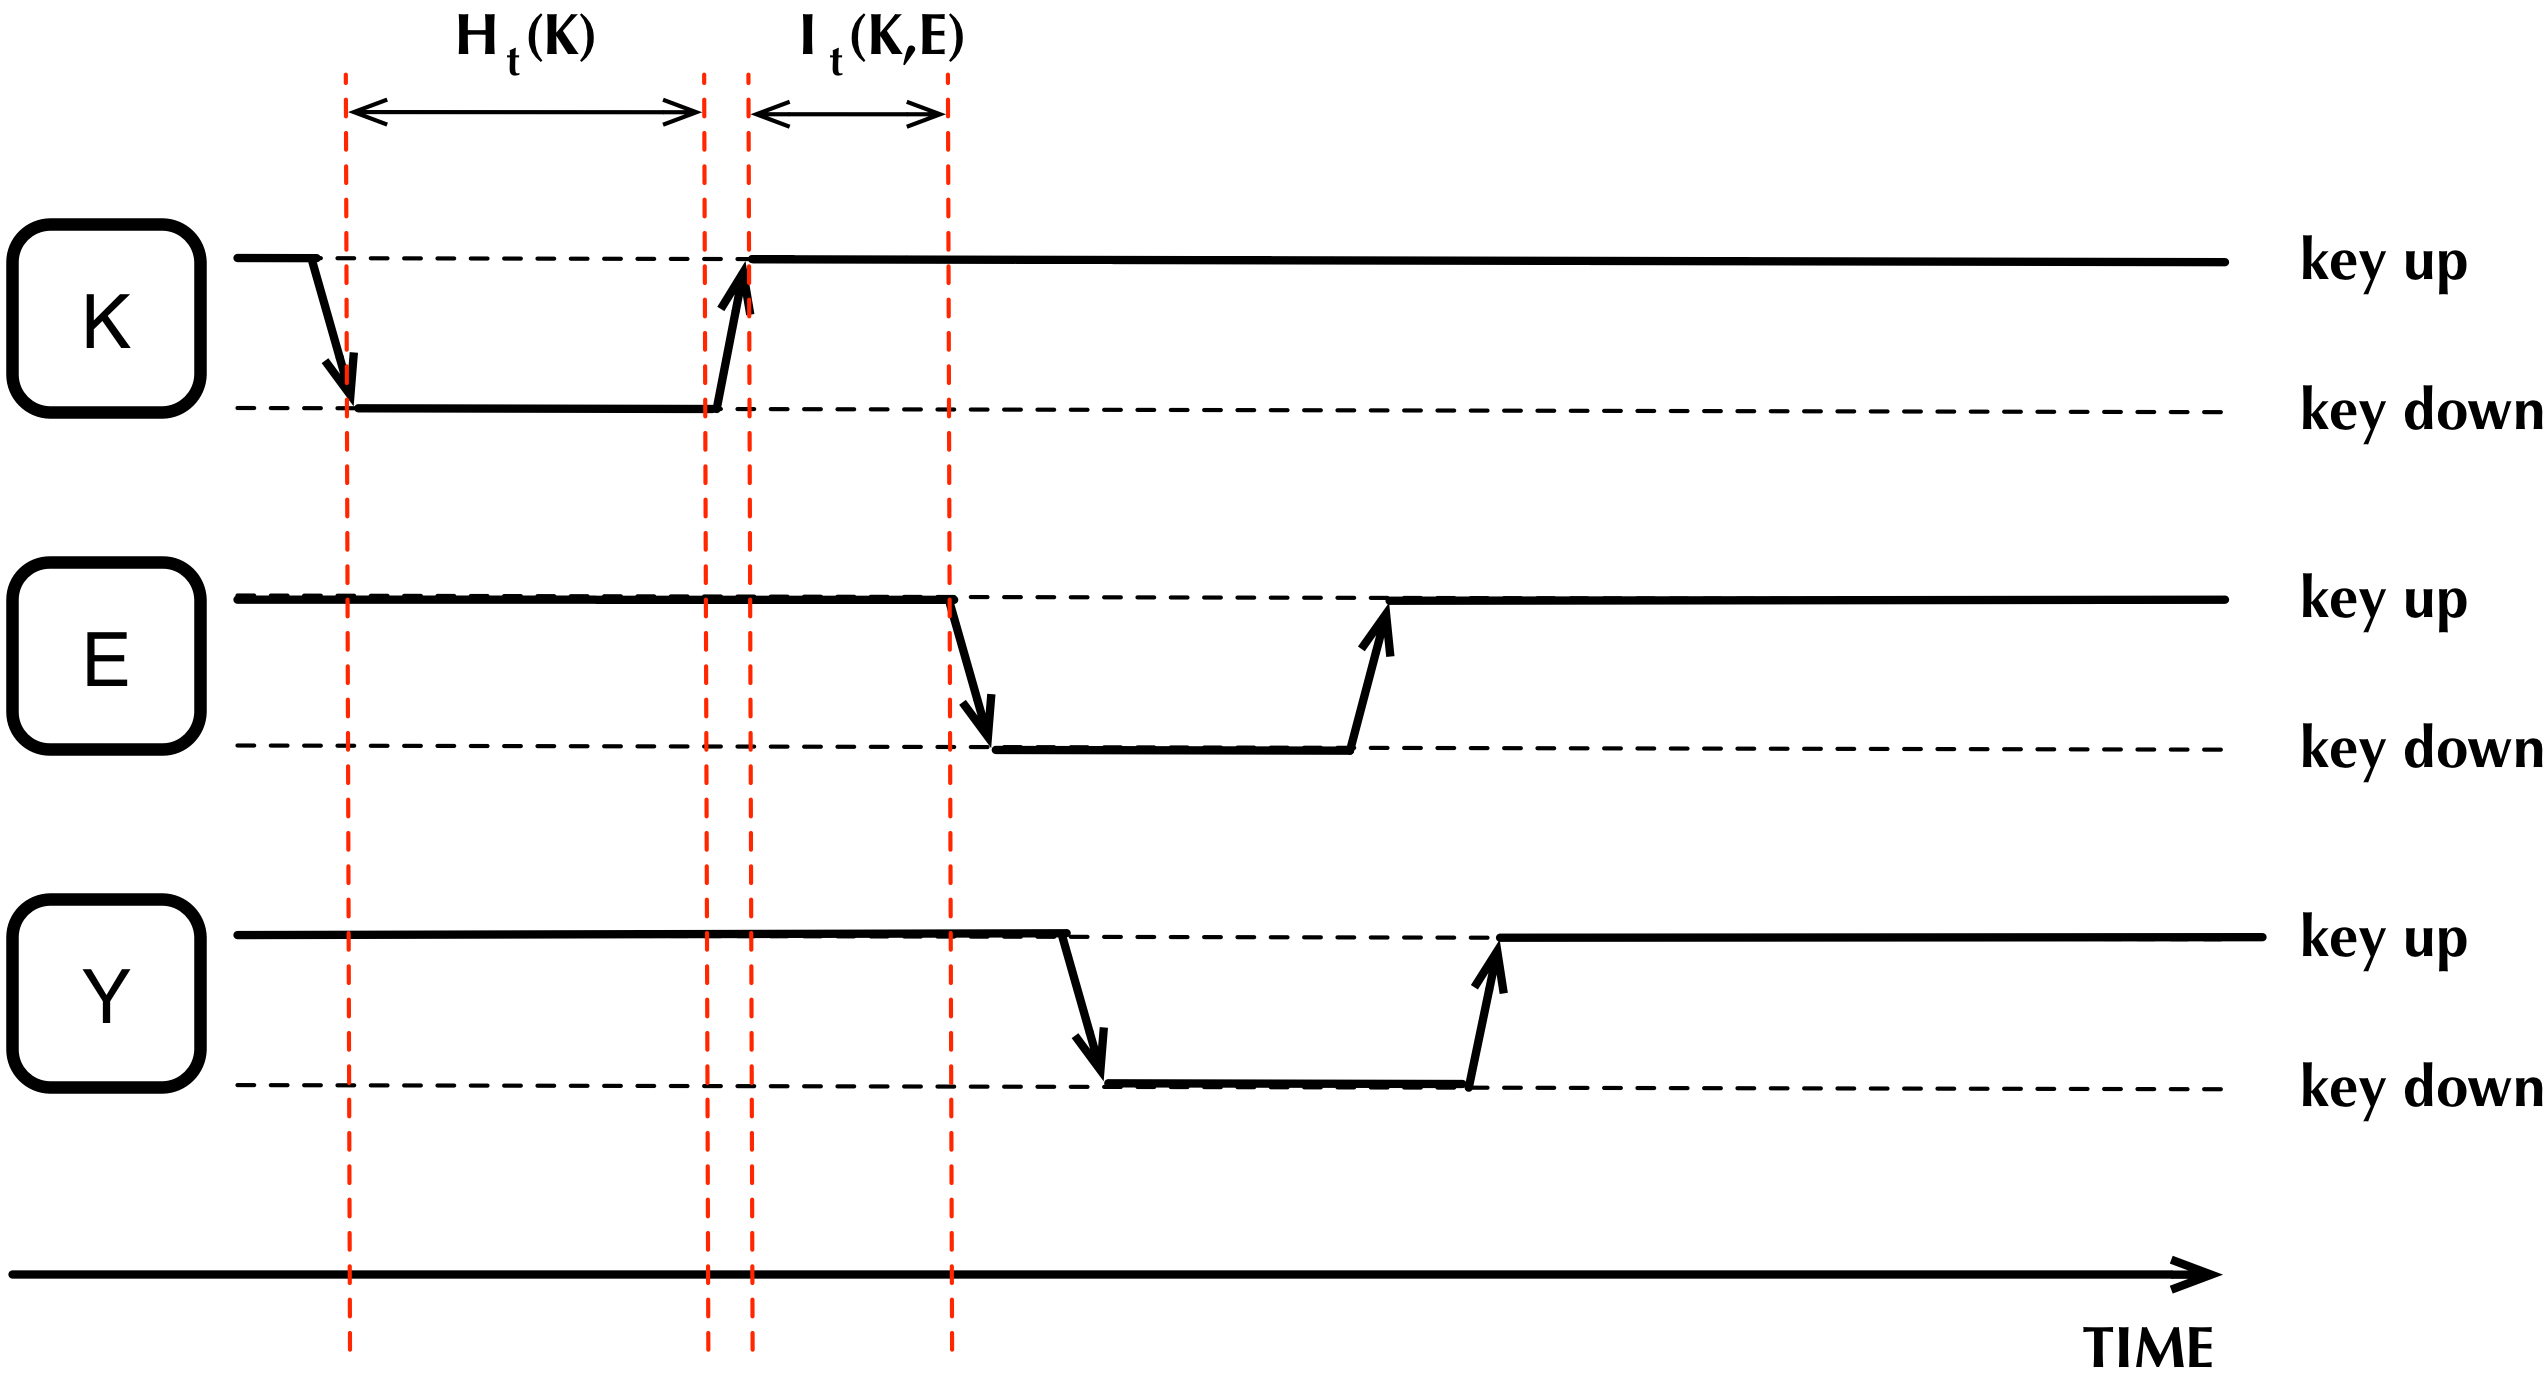
\includegraphics[width=0.70\textwidth]{KeyDyn.png}
\caption{Keystroke Dynamics, adapted from Sim \& Janakiraman \cite{sim2007digraphs}.}
\label{figKD}
\end{figure*}

\subsection{Preprocessing of the Keystroke and Mouse Data}

The raw data obtained from the script needs to be preprocessed to obtain a feature vector.
Basically, this pre-processing consists in measuring the delays between key-
down, key-up or mouse-move events triggered during an assignment.
These events have the dynamic shown in Figure \ref{figKD};
For example when typing the word ‘key’ a
user first presses the letter K and triggers the key-down event, this is
indicated with an arrow that changes the state of the key, the time of the event
is important and also recorded. Only the event data is received from the
browser, in order to generate feature vectors, the patterns and rhythm users
have when pressing consecutive keys are captured measuring the delays between
events, as it is a common practice when dealing with keystroke dynamics. In this
work, the definitions proposed by Sim y Janakiraman \cite{sim2007digraphs} are used. Held
time (Ht) is defined as the time between a key-down and a key-up of the same
key, this would be Ht(K) in the example. Inter key time (It) is defined as the
time between two consecutive key-down events, this time could be negative is the
second key is pressed before the first is released. A sequence is defined as a
list of consecutive keystrokes. In the above example valid sequences could be
[‘K’, ‘E’], [‘E’, ‘Y’] and [‘K’, ‘E’, ‘Y’], the first two are digraphs and the
third is a trigraph. While there can be sequences of any size in a text, working
only with digraphs and trigraphs is preferred. Even if only digraphs and
trigraphs are considered, the amount found in free-text is too large and not
very useful for a feature vector as noted by Epp, Lippold y Mandryk (2007) so
they propose to use statistical measures to capture the patterns; the same
strategy is used in this work. The averages and standard deviations are
calculated from the delays between the events of the digraphs and trigraphs in
each program.


To calculate the average and standard deviations of these key presses, the delays
between a key-down and a key-up event of the left button clicks are used. In
addition to these averages and standard deviations of the delays between
keystrokes and mouse button presses, the average and standard deviations of the
number of total events contained in a digraph and a trigraph are calculated.
These features are proposed and explained by Epp, Lippold y Mandryk \cite{epp2011identifying}. Most
of the times, a digraph should contain four events, while a trigraph six.
However, sometimes an individual can start a digraph or a trigraph before ending
the previous one. These additional features represent these particular cases,
and could be meaningful for the estimation of a learner\'s affective states.
Regarding the mouse movements, the average and standard deviation of the
duration of each mouse movement, and the averages and standard deviations of the
movements in the axes X and Y are also calculated. Lastly, a final feature is
added to preprocessing of the data. The web tutorial recorded  and included in the feature vector how many attempts
a student required before successfully solving an assignment. The final feature vector
consists of 39 features; these are based on the work of Epp, Lippold \& Mandryk
\cite{epp2011identifying} and are shown in Table \ref{tab_features}.

Once feature vectors are obtained from an experiment, the generated dataset is
normally used as training data for a classifier. Researchers of affective
recognition have used a wide variety of classification algorithms. As a proof of
concept four well known classification algorithms where compared: k-Nearest
Neighbors (k-NN) algorithm, a feed forward neural network trained with back-
propagation, a na\"ive Bayes classifier and finally a decision trees algorithm for
rational data (J-48) \cite{tan2006introduction}. Experiments and results will be presented next.

\section{Experiment and results}
\label{sec:exp}
The aim of this research is to evaluate the use of keyboard
and mouse dynamics as an appropriate sensory input for an affective recognition
system in a learning environment for programmers,
who interactively write short programs. An experimental approach was adopted with this aim: Sensory and
quantitative data was collected from learners as they were enrolled in a basic
course of Python programming. This data was then pre-processed using the method
described earlier in Section \ref{sec:method}, and together with the quantitative data obtained from users,
classifiers were trained and validated. The results were then compared
and we arrived to some conclusions regarding the effectiveness of the method. The goal given to
subjects was to solve as many assignments as they could in a period of two weeks.
There was neither time limit nor a minimum amount of time required for a
participant while trying to solve the assignments or complete the tutorial. The
participants were able to stop and resume their interaction with the system at
any time.
%
\begin{figure*}[!t]
\centering
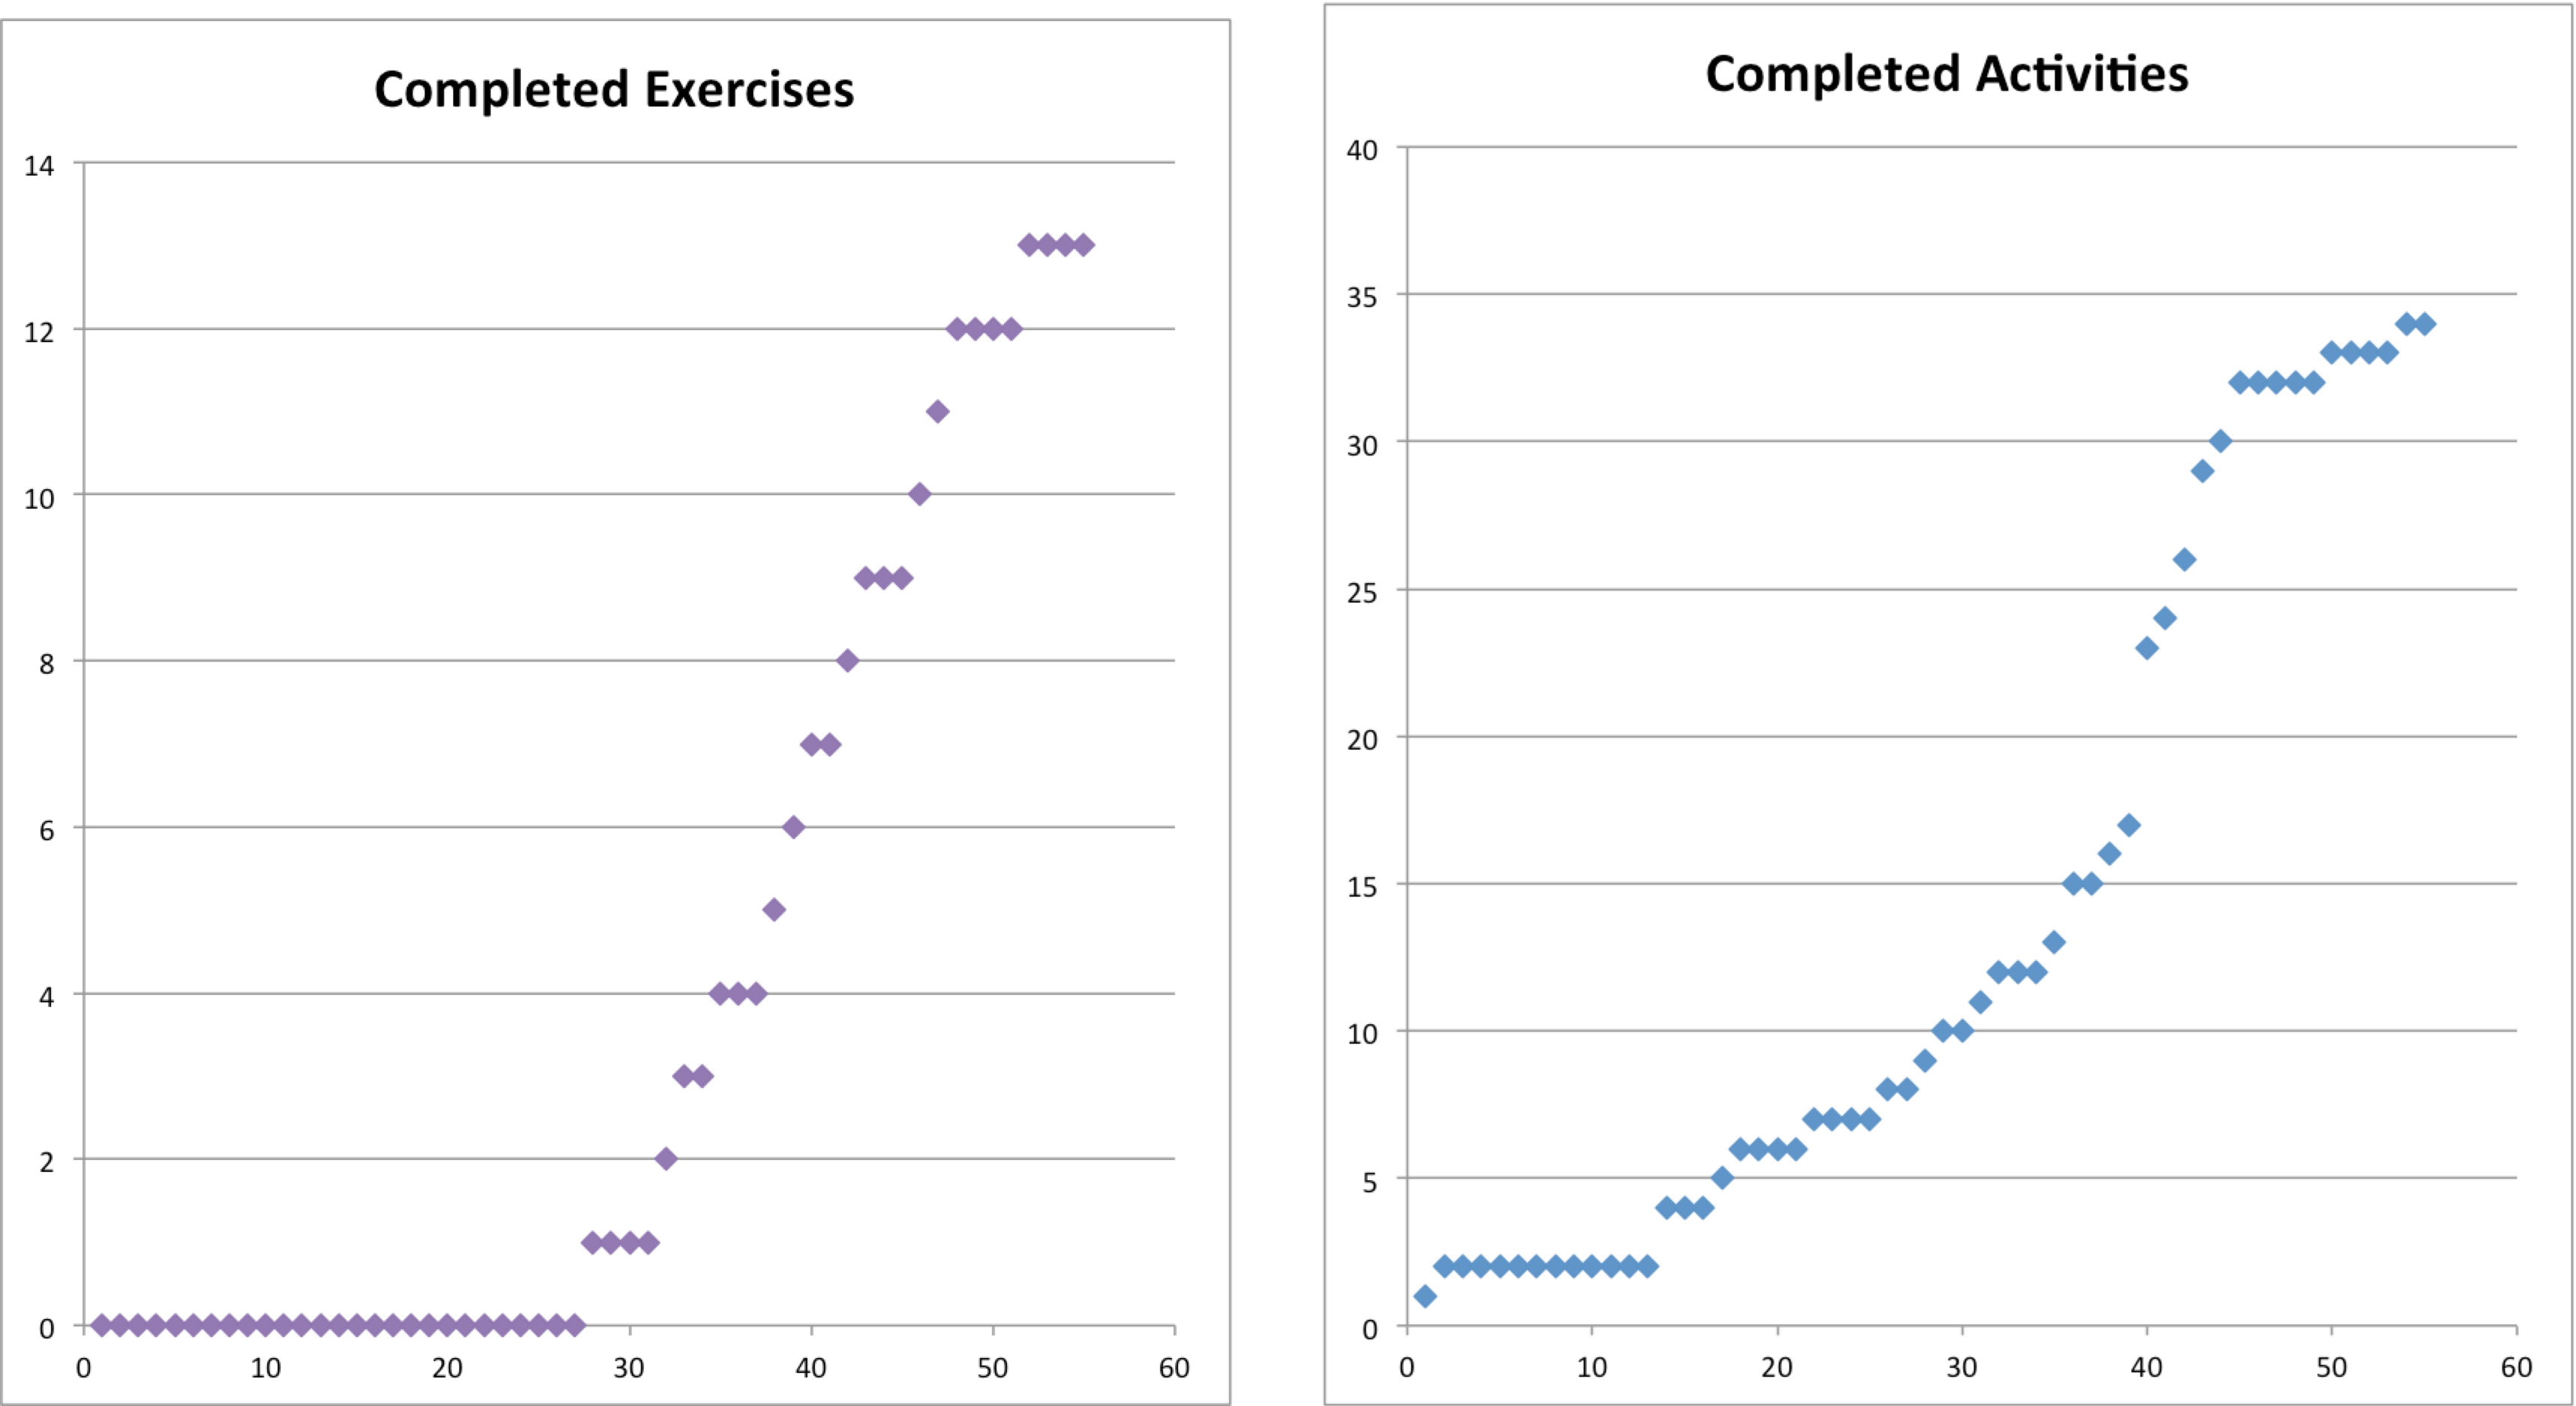
\includegraphics[width=0.48\textwidth]{Completed.png}
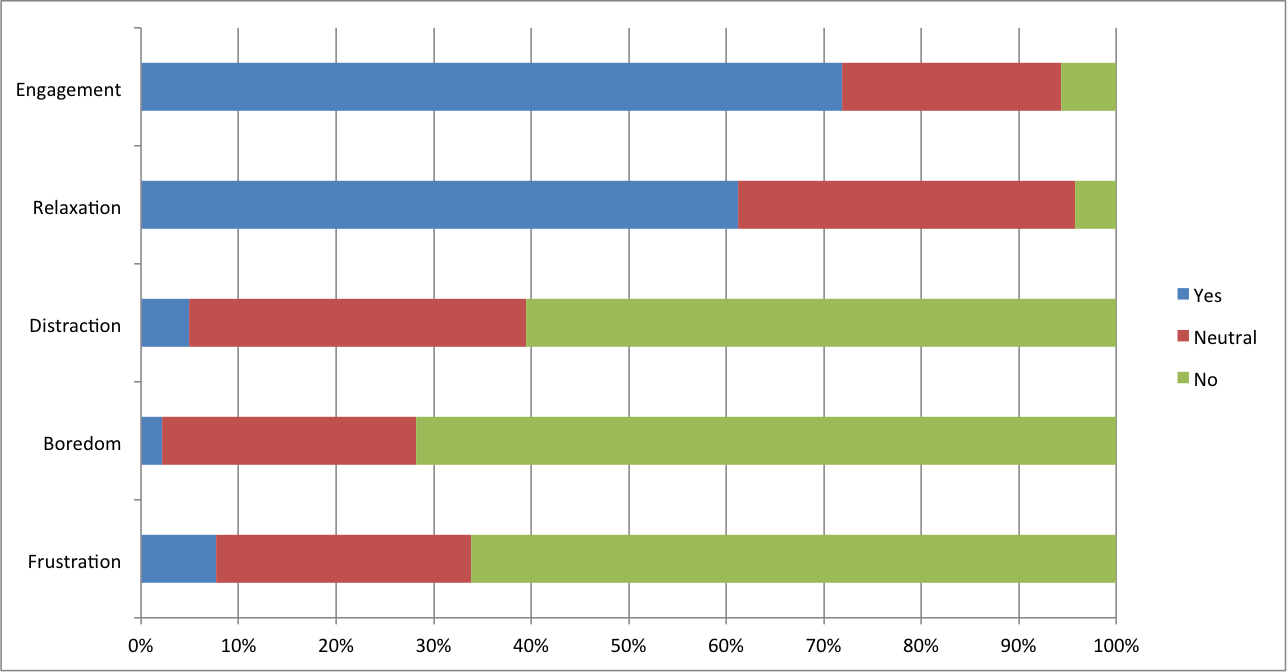
\includegraphics[width=0.48\textwidth]{classDist.png}
\caption{Completed activities and assignments by learner in ascending order (left) and distribution of emotions reported (right) \cite{ijcci17}.}
\label{fig_completed}
\end{figure*}

A tutorial was developed to
obtain the necessary data using the proposed platform Protoboard, a web-based environment,
whose latest version has been released under an open source license,
and can be found online at \url{https://github.com/mariosky/protoboard}.
The main functionality  used for this experiment is
shown schematically in Figure \ref{fig_process} . % Don't know what's
                                % happened to this  
                                % There it was.
Users log in to
Protoboard  by creating an account or by using their account 
credentials from the
social network Facebook. The web tutorial begins with three introductory 
videos that explain
the fundamentals of programming in Python, and how to use the editor to
execute their code. What follows after these videos, are 13 programming
assignments that students need to solve in sequential order. Assignments are of
incremental difficulty.
In Figure \ref{fig_editor},
the user interface of the programming editor is
presented.
For this experiment Protoboard was configured to allow unlimited
attempts to solve each assignment.

A total of 55 volunteers, with no previous experience in Python, where recruited
as a response to three announcements in a special interest group of programming
students in a social network, but the fact that they needed Facebook kept some prospects from
volunteering; a subject reported that he normally creates temporary email
accounts to try new web services; however, the use of Facebook gave researchers access to public
information about the subjects. Their ages were in the range of 18 to
30 years. Although no experience in software programming was needed, as the
web tutorial\'s course is of a very basic level, participants had
different levels of experience, from 0 (8 persons) to more than 5 (22).

\begin{table}[!t]
\centering
\caption{ Survey question: How many years of programming experience do you have? }
\label{tab_results}
    \begin{tabular}{ | c | l | }
    \hline
    Years Programming          & Number of Learners \\
    \hline
   		0   &  8 \\
    \hline
    	1   &  13\\
    \hline
    	2-4  & 15\\
    \hline
    	5+   & 22\\
    \hline
    \end{tabular}

\end{table}


\begin{table*}[!t]
\centering
\caption{Performance of every classifier with 10-fold cross validation \cite{ijcci17}. Each cell shows accuracy and ($\kappa$)}
\label{tab_performance}
    \begin{tabular}{ | c | l | l | l | l | }
    \hline
    Affect          & Na\"ive Bayes           & J-48                & k-NN              & ANN \\
    \hline
    Flow/engaged    & 79.00\% (0.50) & 80.48\% (0.51) & 76.14\% (0.43) & 78.43\% (0.45) \\
    \hline
    Relaxation      & 71.10\% (0.40) & 72.57\% (0.45) & 69.14\% (0.37) & 71.24\% (0.34)\\
    \hline
    Distraction     & 70.33\% (0.43) & 71.00\% (0.43) & 74.00\% (0.50) & 72.52\% (0.39)\\
    \hline
    Frustration     & 74.71\% (0.49) & 73.86\% (0.45) & 72.62\% (0.42) & 78.00\% (0.50)\\
    \hline
    Boredom         & 74.71\% (0.47) & 84.57\% (0.59) & 83.81\% (0.58) & 76.19\% (0.45)\\
    \hline
    \end{tabular}
\end{table*}



\begin{table*}[!t]
\centering
\caption{Performance of classifiers for Flow/Engaged  with 10-fold cross validation and optimized feature-weights }
\label{tab_perf_flow}
    \begin{tabular}{ | l | l | l | }
    \hline
    Classifier   &  Accuracy            & $\kappa$                 \\
    \hline
    Na\"ive Bayes     & 72.52\%  & 0.339  \\
    \hline
    Deep Neural Network     & 78.29\%  & 0.419  \\
    \hline
    Random Forest      & 78.81\%  & 0.360  \\
    \hline
    Gradient Boosted Trees     & 78.95\%  & 0.415  \\
    \hline
    KNN      & 76.19\%  & 0.242  \\
    \hline
    Na\"ive Bayes Kernel     & 80.22\%  & 0.346 \\
    \hline
    J48     & 78.19 \%  & 0.433  \\
    \hline
  
    \end{tabular}
\end{table*}



In order to determine what affective states a student was experiencing, the
Experience Sampling Method (ESM) \cite{kubey1996experience} was used.
After the students successfully solve a programming assignment, they were presented
with an ESM survey that asks what they were feeling during their solving of the
assignment. A very brief description is given about what to do in this survey,
followed by statements the students need to answer according to how they were
feeling. As an example, the statement “I was feeling frustrated” is presented,
and a student needs to answer either “Strongly agree,” “Agree,” “Neutral,”
“Disagree,” and “Strongly Disagree.”

After the two weeks of the experiment, only four learners completed all of the
programming assignments and 22 did not completed any. Out of the total activities
available (videos, survey and questionnaires) only two completed all. Figure \ref{fig_completed}
shows the number of assignments and activities completed by each learner.

The participants\' interaction generated a total of 142 feature vectors one for each
successfully completed assignment. The affective states reported by learners after
completing each assignment was grouped in three classes: ‘Yes’, ‘Neutral’ and
‘No’. The class distribution of the emotions reported is shown in Figure 6. This
results show that the most common emotions were flow/engagement (72\%) and
relaxation (61\%) while few learners reported distraction (5\%), frustration
(8\%) and boredom (2\%). This distribution is different from what was reported
by D\'Mello et al. \cite{bixler2013detecting} and Rodrigo et al. \cite{rodrigo2009affective}.
Although Flow/Engagement was
also the predominant class, the distribution is skewed to the first two. There
are some possible reasons for this; first the majority of students had
prior experience in programming, so learning new one is not that problematic, a second
reason could be the freedom users had to abandon the activities, perhaps
frustrated or bored learners simply quit the tutorial. A high number of learners
(49\%) did not completed any assignment and the once who completed more where also
the more experienced.

\begin{table}[h!tb]
\centering
\caption{Parameters used in the evolutionary algorithm for feature
  selection.}
\label{tab_ga}
    \begin{tabular}{ | l | l | }
      \hline
      Parameter & Value \\
      \hline
      Population size & 700 \\
      Generations & 30 \\
      Selection & Tournament \\
      Tournament size & population size / 4 \\
      Crossover & Uniform \\
      Crossover probability & 0.5 \\
      Mutation rate & $1 \over 39$ \\
      Minimum number of features & 5 \\
            \hline

    \end{tabular}
  \end{table}
  
As part of the data mining process a canonical genetic algorithm was used for feature
selection with the parameters used shown in Table \ref{tab_ga}. These
parameters were set heuristically, and were the same for selecting the
features of all classification algorithms. % Mario check this - JJ
In the end, the subset for the frustration classifier includes only 11 features, and 
the subset for the boredom classifier consists of only 13 features. 

% It's not clear what's the fitness function here or what it really does. Maybe we could expand this part of the work, test different evolutionary algorithms and write a paper on feature selection using evolutionary algorithms for EvoStar - JJ

The selected classifiers where implemented using Rapid Miner, with the
following parameters: For J48 decision tree algorithm a confidence threshold
for pruning of 0.25, with a minimum of 2 instances per leaf, and 3 folds for
reduced error pruning. The feed-forward neural network used a back-propagation
learning algorithm with two hidden layer of 20 neurons each, with a learning
rate and momentum of 0.6, and was trained for 200 generations.

Table \ref{tab_performance} shows the performance of each of the four
classifiers together
with the $\kappa$ coefficients. A 10-Fold cross validation was used.
The accuracies and $\kappa$ coefficients obtained are close to what is
usually obtained in fixed-text methods, for example, the results presented in
Epp, Lippold y Mandryk \cite{epp2011identifying}.
In a fixed-text method, subjects are asked to write specific texts.
The results obtained with this method are satisfactory, considering that
learners were writing a program, a task comparable with free-text writing,
where there is no restriction on what has to be written.
In the case of the $\kappa$ coefficients, it is
usual to see values below 0.2 in methods involving free-text. In this case, some
values of $\kappa$ were close to 0.5, is important to consider the values of $\kappa$
in these results because the class distribution is not uniformly distributed. As
it is observed in many works in affective recognition, decision trees normally
produce competitive accuracy. In this case the J-48 classifier obtained an
accuracy of 80.48\%, which is marginally better than the others, and an accepted $\kappa$
statistic for the kind of problem. The artificial neural network (ANN)
gives the highest
accuracy in the classification of frustration.
%
\begin{table}[h!tb]
\centering
\caption{Parameters used in the evolutionary algorithm for feature
  weight optimization.}
\label{tab_ga_w}
    \begin{tabular}{ | l | l | }
      \hline
      Parameter & Value \\
        \hline
      Population size & 10 \\
      Generations & 30 \\
      Selection & Tournament \\
      Tournament size & population size / 4 \\
      Crossover & Uniform \\
      Crossover probability & 0.5 \\
      Mutation rate & $1 \over 39$ \\
      Minimum number of features & 5 \\
        \hline
    \end{tabular}
  \end{table}
% 
\begin{table*}[!t]
\centering
\caption{Parameters used for the different classification algorithms }
\label{tab_params_ml}
\label{tab_perf_flow}
    \begin{tabular}{ | l | l |  }

      Algorithm & Parameters \\
      \hline
    \end{tabular}
  \end{table*}
      
Table \ref{tab_perf_flow} shows the performance for the additional classifiers
evaluated specifically for the Flow/engaged affective state. The goal was to
increase the performance achieved earlier. Again a ten-
fold cross-validation was conducted. In this case, instead of using an
evolutionary algorithm to optimize feature selection, it was used for 
optimizing a weight vector. 
      The feature-weight vector assigned a weight to each one of the
      features, and the parameters that have been used in the
      evolutionary algorithm are shown in Table \ref{tab_ga_w}.
      % The
% parameters used for the evolutionary optimization algorithm are the following:
% Population size = 10, generations = 30, selection = tournament, tournament size = 0.25 (fraction of the population),  initialize probability = 0.5,  mutation
%       probability = 1/number of attributes,  crossover probability =
%       0.5.
      % Please Mario check these parameters and how they have put to
      % the table; I don't know what's the "initialization
      % probability" - JJ

      Parameters
used for the Random Forest algorithm: number of trees = 10, 
criterion = gain ratio, maximal depth = 20, 
confidence = 0.25, minimal gain = 0.1, minmail leaf size = 2.  The
parameters used for are the J48 are the following:  confidence = 0.79, minimal
leaf size=2. For the kNN algorithm, the value k = 4 was used. 
For gradient boosted
trees: number of trees = 20,  maximal depth = 5, minimum rows = 10, 
minimum split 
improvement = 0.0, number of bins = 20, 
learning rate = 0.1, sample rate = 1.0.  Bayes
Kernel: laplace correction = True, estimation mode = greedy, 
minimum bandwidth = 0.1, number of kernels = 10.  Finally for deep learning: activation = Rectifier, hidden layer sizes = [50, 50], epochs = 10. 


Again the accuracy and $\kappa$ values of the
algorithms show the difficulty of having classes that are not uniformly
distributed, with several algorithms reaching an acceptable accuracy but with a
low value of  $\kappa$, this is an indication of algorithms classifying almost
everything as the dominant class. The results of the tree induction algorithms
are better when we consider both accuracy and  $\kappa$ values. In the case of
kernel-based or deep learning methods they provide competitive results but at a
higher computational cost.
 

\section{Conclusion}

The aim of this research was to evaluate the use of keyboard and mouse dynamics
as an appropriate sensory input for an affective recognition system. The context
of use is a learning environment for programmers, in particular for learning
assignments consisting in writing short programs interactively. An experimental
approach was adopted with this objective, by effectively using the
method with real subjects using the environment.

The proposed method in this work obtained
satisfactory results. It is usual for a classification method based on free-text
to obtain an accuracy and $\kappa$ measure below their counterparts of
fixed-text; however, in this
work the results obtained were similar to those works applied to fixed-text
dynamics. A possible explanation of this would be the addition of the mouse
dynamics features and the additional preprocessing performed on the
feature vectors.  Out of all methods tested, tree induction algorithms
obtained better results when we take into consideration both accuracy and  $\kappa$ values.

While these are promising results further experiments are
needed. Other experiments should focus on novice programmers, with
which we expect to gather more data and more representative examples for all the
clasess. These experiments should give researchers the hability to do stratified samples to balence
the class distribution and achieve better results. Also more experiments should
give more insigth on the relationship between affective state  and interactive
behavior. Results show near 80\% accuracy, these results  are competitive
against other classifiers of a similar domain, but we do not know yet what is
the effectiveness when applied to affective-aware learing environments.   

%This
% But you have to comment on how this addresses the problem. Which
% should be in the title that is not there yet - JJ
% You also have to draw a _hard_ conclusion. Is programming using free
% text better than what? Typing a fixed text?
% Is 80% effective?
%  - done  Mario 
Future work will focus on extracting other features from the learners\' interaction such as behavioral data, as proposed by Blikstein
\cite{blikstein2011using}; the parameters proposed by this author
include the size of the program and changes in the code. Other authors
also propose treating the use of certain keys as features e.g., the
delete key because it is mainly used for correcting sentences. Also a multi-modal approach is needed. Since all these need a completely new approach, a new methodology will be developed to
gather data and take measures.

% use section* for acknowledgment
\section*{Acknowledgment}
This work has been supported in part by: de Ministerio espa\~{n}ol de
Econom\'{\i}a y Competitividad under project TIN2014-56494-C4-3-P
(UGR-EPHEMECH),  DeepBio (TIN2017-85727-C4-2-P) and by CONACYT PEI Project No. 220590.

\bibliographystyle{apalike}
% argument is your BibTeX string definitions and bibliography database(s)
\bibliography{programming}

\vfill
\end{document}
